% Original schematic. Square 7.055-inch canvas, native-size vector labels.
\RequirePackage{fix-cm}
\documentclass[tikz,border=0pt]{standalone}
\usepackage[T1]{fontenc}
\usepackage{helvet,amsmath,amssymb}
\usetikzlibrary{arrows.meta,calc,decorations.pathreplacing}
\renewcommand{\familydefault}{\sfdefault}
\pdfinfoomitdate=1
\pdftrailerid{}
\pdfsuppressptexinfo=15
\definecolor{ink}{HTML}{202A35}
\definecolor{muted}{HTML}{6B7785}
\definecolor{line}{HTML}{CCD4DC}
\definecolor{blue}{HTML}{2769B0}
\definecolor{teal}{HTML}{138A83}
\definecolor{orange}{HTML}{D57525}
\begin{document}
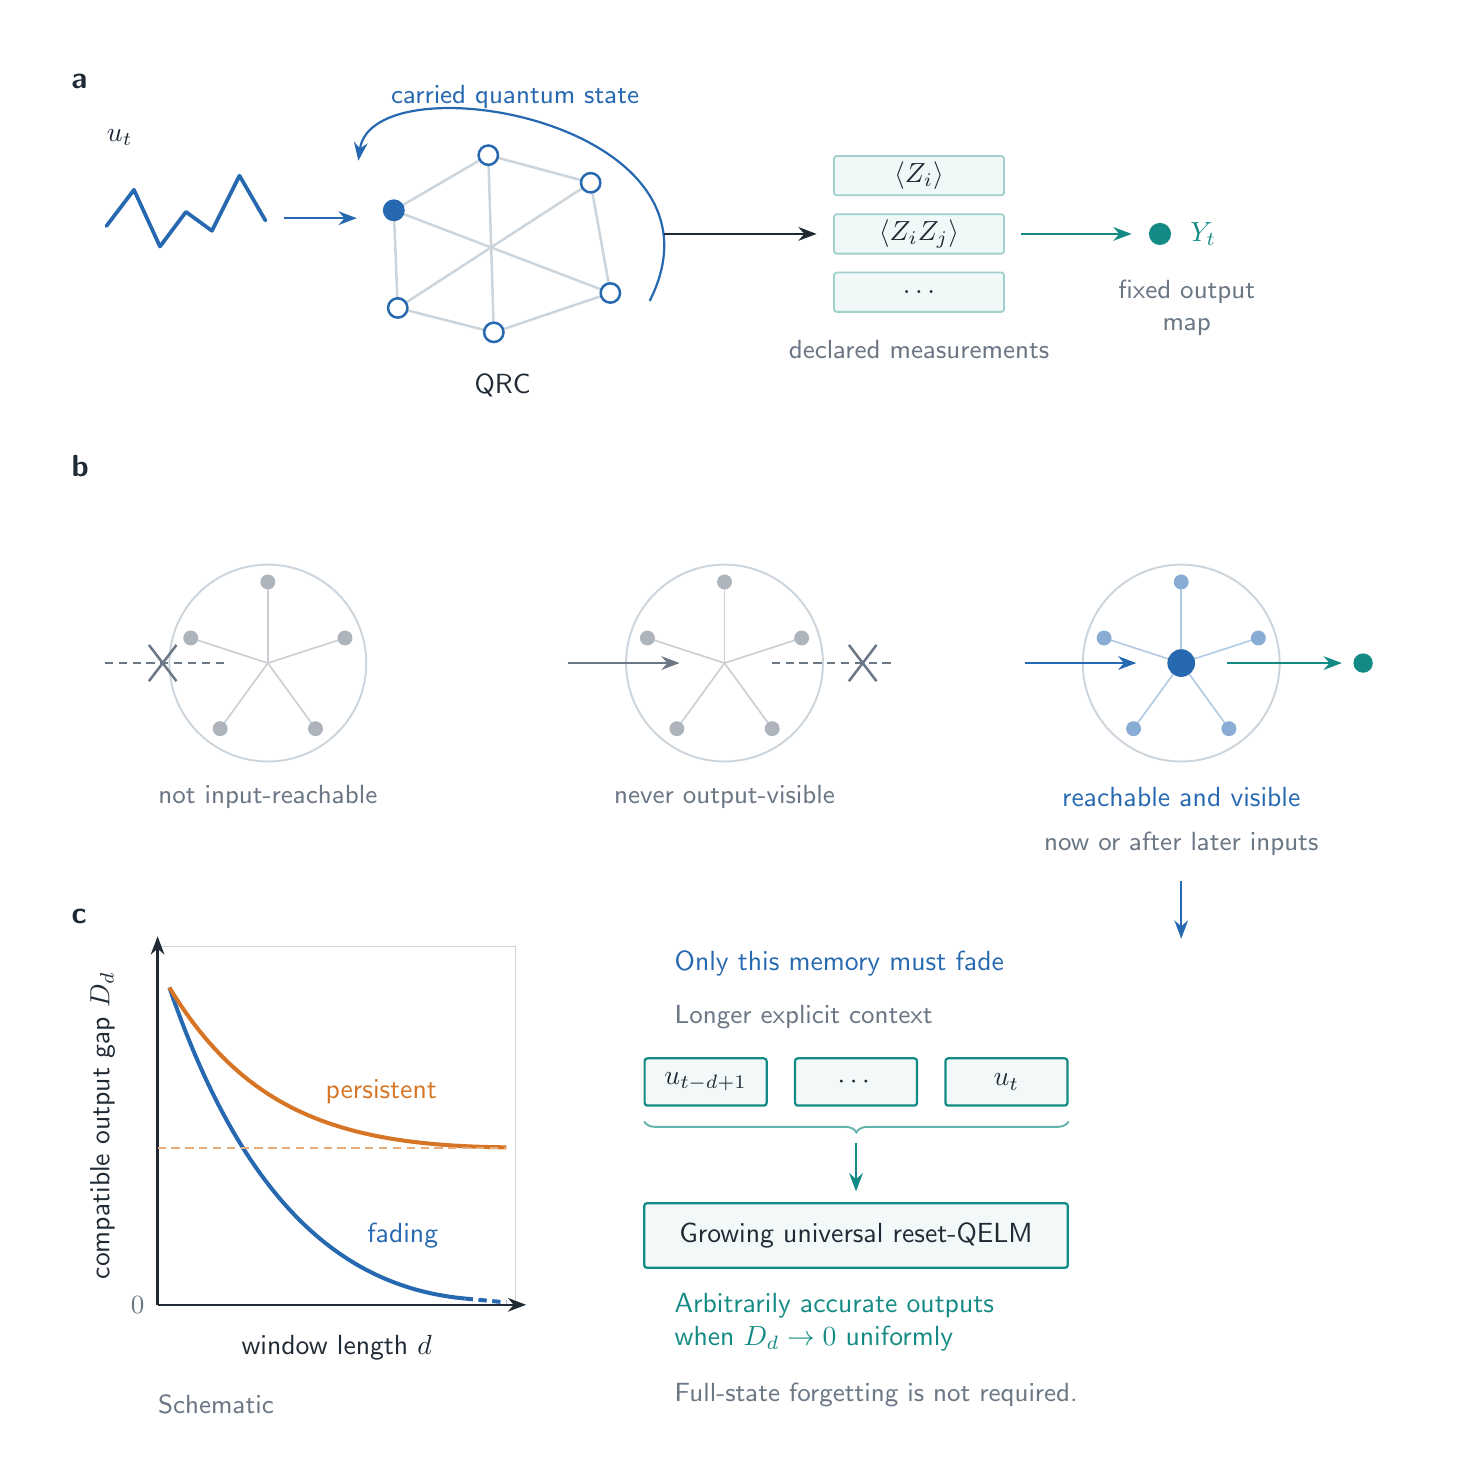
\begin{tikzpicture}[
 x=1cm,y=1cm,
 every node/.style={font=\fontsize{10}{12}\selectfont,text=ink,inner sep=0pt},
 >={Stealth[length=4.6pt,width=3.4pt]},
 arrow/.style={-{Stealth},line width=.8pt,draw=ink},
 edge/.style={draw=line,line width=.9pt},
 dot/.style={circle,draw=blue,fill=white,line width=.9pt,minimum size=7pt},
 tag/.style={anchor=west,font=\fontsize{11}{13}\selectfont\bfseries},
 note/.style={text=muted,font=\fontsize{9.5}{11.5}\selectfont},
 gate/.style={draw=teal,line width=.8pt,rounded corners=1pt,fill=teal!5,
              minimum width=1.18cm,minimum height=.6cm}
]
\path[use as bounding box] (0,0) rectangle (17.9197,17.9197);

% a: input, physical recurrent state, declared measurements.
\node[tag] at (.55,17.23) {a};
\node[anchor=west] at (1.00,16.52) {$u_t$};
\draw[blue,line width=1.35pt,line cap=round,line join=round]
 (1.0,15.40)--(1.35,15.86)--(1.68,15.14)--(2.01,15.58)--(2.34,15.34)
 --(2.69,16.04)--(3.02,15.47);
\draw[arrow,blue] (3.25,15.5)--(4.18,15.5);
\foreach \name/\x/\y in {p/4.65/15.60,q/5.85/16.30,r/7.15/15.95,
 s/7.40/14.55,v/5.92/14.05,w/4.70/14.36}{\coordinate (\name) at (\x,\y);}
\foreach \start/\end in {p/q,q/r,r/s,s/v,v/w,w/p,p/s,q/v,r/w}
 \draw[edge] (\start)--(\end);
\foreach \name in {p,q,r,s,v,w}{\node[dot] at (\name) {};}
\fill[blue] (p) circle (3.6pt);
\draw[arrow,blue] (7.90,14.45).. controls (9.06,16.75) and (4.37,17.52)..(4.20,16.23);
\node[note,text=blue] at (6.19,17.04) {carried quantum state};
\node at (6.03,13.38) {QRC};
\draw[arrow] (8.08,15.30)--(10.02,15.30);
\foreach \yy/\txt in {16.04/{$\langle Z_i\rangle$},15.30/{$\langle Z_iZ_j\rangle$},14.56/{$\ldots$}}{
 \draw[teal!40,fill=teal!6,line width=.65pt,rounded corners=1pt]
   (10.24,{\yy-.25}) rectangle (12.40,{\yy+.25});
 \node at (11.32,\yy) {\txt};
}
\node[note] at (11.32,13.83) {declared measurements};
\draw[arrow,teal] (12.62,15.3)--(14.02,15.3);
\fill[teal] (14.38,15.30) circle (4pt);
\node[anchor=west,text=teal] at (14.76,15.3) {$Y_t$};
\node[note,align=center] at (14.72,14.36) {fixed output\\map};

% b: a visual filter on state differences, not all-state erasure.
\node[tag] at (.55,12.35) {b};
\foreach \xx/\col in {3.05/muted,8.85/muted,14.65/blue}{
 \draw[line,line width=.7pt] (\xx,9.85) circle (1.25cm);
 \foreach \ang in {18,90,162,234,306}{
  \draw[\col!35,line width=.6pt] (\xx,9.85)--++(\ang:1.03cm);
  \fill[\col!55] ($(\xx,9.85)+(\ang:1.03cm)$) circle(2.7pt);
 }
}
\draw[muted,densely dashed,line width=.85pt] (.98,9.85)--(2.50,9.85);
\draw[muted,line width=.9pt] (1.54,10.08)--(1.89,9.62) (1.54,9.62)--(1.89,10.08);
\node[note] at (3.05,8.15) {not input-reachable};
\draw[arrow,muted] (6.86,9.85)--(8.28,9.85);
\draw[muted,densely dashed,line width=.85pt] (9.45,9.85)--(11.0,9.85);
\draw[muted,line width=.9pt] (10.43,10.08)--(10.78,9.62) (10.43,9.62)--(10.78,10.08);
\node[note] at (8.85,8.15) {never output-visible};
\draw[arrow,blue] (12.67,9.85)--(14.08,9.85);
\fill[blue] (14.65,9.85) circle(5pt);
\draw[arrow,teal] (15.23,9.85)--(16.69,9.85);
\fill[teal] (16.96,9.85) circle(3.5pt);
\node[text=blue] at (14.65,8.15) {reachable and visible};
\node[note,align=center] at (14.65,7.55) {now or after later inputs};
\draw[arrow,blue] (14.65,7.08)--(14.65,6.35);

% c: square schematic axis and its operational interpretation.
\node[tag] at (.55,6.63) {c};
\begin{scope}[shift={(1.65,1.70)}]
 \draw[line,line width=.45pt] (0,4.55)--(4.55,4.55)--(4.55,0);
 \draw[arrow] (0,0)--(4.68,0);
 \draw[arrow] (0,0)--(0,4.68);
 \node[rotate=90] at (-.70,2.275) {compatible output gap $D_d$};
 \node at (2.275,-.54) {window length $d$};
 \node[note,anchor=east] at (-.16,0) {$0$};
 \draw[blue,line width=1.45pt] (.15,4.03).. controls (1.12,1.20) and (2.42,.22)..(3.90,.08);
 \draw[blue,densely dashed,line width=1.45pt] (3.90,.08)--(4.43,.03);
 \draw[orange,line width=1.45pt] (.15,4.03).. controls (1.12,2.43) and (2.36,2.02)..(4.43,2.00);
 \draw[orange!60,densely dashed,line width=.7pt] (0,1.99)--(4.43,1.99);
 \node[anchor=west,text=orange,inner sep=1.6pt] at (2.07,2.70) {persistent};
 \node[anchor=west,text=blue,inner sep=1.6pt] at (2.60,.88) {fading};
\end{scope}
\node[note,anchor=west] at (1.65,.44) {Schematic};

\node[anchor=west,text=blue] at (8.21,6.04) {Only this memory must fade};
\node[anchor=west,note] at (8.21,5.35) {Longer explicit context};
\foreach \xx/\txt in {8.61/{$u_{t-d+1}$},10.52/{$\cdots$},12.43/{$u_t$}}{
 \node[gate,minimum width=1.55cm] at (\xx,4.53) {\txt};
}
\draw[teal!65,line width=.7pt,decorate,decoration={brace,mirror,amplitude=4pt}]
 (7.83,4.03)--(13.22,4.03);
\draw[arrow,teal] (10.52,3.76)--(10.52,3.14);
\node[gate,minimum width=5.38cm,minimum height=.82cm] at (10.52,2.58)
 {Growing universal reset-QELM};
\node[anchor=west,align=left,text=teal] at (8.21,1.48)
 {Arbitrarily accurate outputs\\when $D_d\to0$ uniformly};
\node[anchor=west,note] at (8.21,.56) {Full-state forgetting is not required.};
\end{tikzpicture}
\end{document}
